%\chapter{プロジェクトの進め方}
\section{進め方の概要}
本プロジェクトでは、PDCAサイクル、スクラムなどのアジャイルソフトウェア開発の手法を学び、実践しながらアプリケーションを開発した。以下に大まかな年間スケジュールを示す。まず、5月にGit、Swift勉強会を通じ、プロジェクトを進めるうえで欠かせない実装力を身につけた。また、同時期に第1回木古内フィールドワークも行い、開発するアプリケーションの要件定義を進めていった。6月からは本格的に開発に着手し、より詳細な要件定義やアプリケーションの設計、実装から評価、改善点の検討までの一連の流を前期中に2回行った。後期も同様に開発を進め、最終成果発表の時点では1年を通して合計で4回の開発を行うことができた。
\begin{figure}[htbp]
  \begin{flushleft}
    \begin{tabular}{c}

      % 1
      \begin{minipage}{0.7\hsize}
        \begin{center}
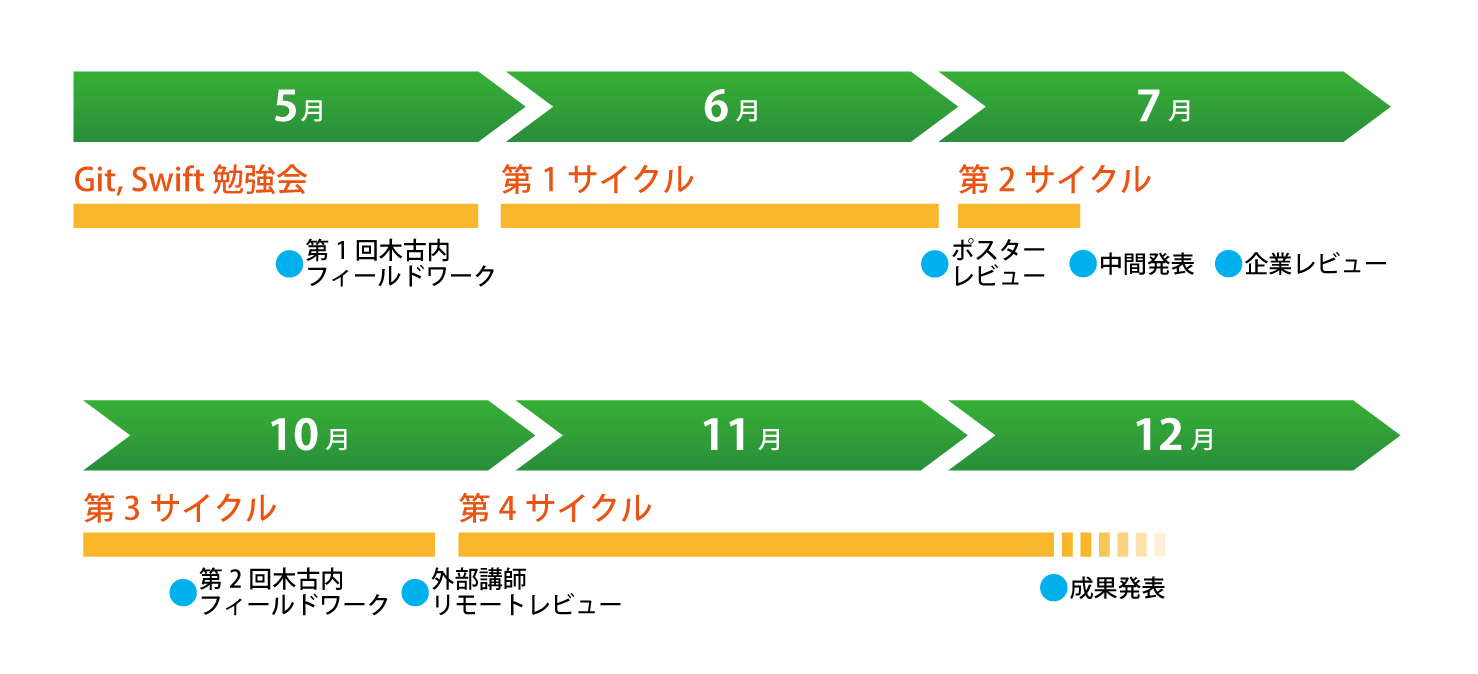
\includegraphics[width=15cm, bb=0 0 1478 674]{procedure-1.png}
       
        \end{center}
      \end{minipage}

    \end{tabular}
    \caption{年間スケジュール}
    \label{fig:lena}
  \end{flushleft}
\end{figure}


\bunseki{横山翔栄}

\section{開発の進め方}
PDCAサイクルの「計画、実行、評価、改善」の各フェーズについて、本プロジェクトで実践した内容について記述する。
\subsection{計画(Plan)フェーズ}
各サイクルの初めに、どのようなアプリケーションを開発するかを計画した。計画にあたっては、開発するアプリケーションの新規性や、ターゲットユーザにもたらすメリットなどを検討し、実際に役立つアプリケーションになるよう繰り返し話し合った。以下に本プロジェクトグループが計画フェーズで用いたツールや手法について記述していく。
\subsubsection{リーンキャンバス}
アプリケーションの開発のためのアイデアを9種類の要素を用いて整理することで、より綿密な要件定義を行うことができた。ただし、今回のプロジェクトにおいてはビジネス化が目的ではないため、コストについての検討は行わなかった。
\subsubsection{プロトタイプ}
本格的な開発に着手する前に、簡易なモデルを作成して検討することで、問題点や改善案を挙げることができた。プロトタイピングは各サイクルでのアプリケーションの機能に関わる部分をSwiftで作成したのに加え、第3サイクルではカルタを、第4サイクルではリーフレットをAdobe Illustratorで作成し実際に印刷し、検討を重ねた。実際に作成したプロトタイプについては図5.6、図5.7を参照していただきたい。
\subsection{実行(Do)フェーズ}
実行フェーズでは、計画フェーズで行った要件定義やアプリケーション設計をもとに、実際に開発を進めていく。以下に、本プロジェクトで実践したソフトウェア開発の手法について記述していく。
\subsubsection{スクラム}
前節でも述べたとおり、メンバのタスク管理にはスクラムを用いた。まず、次バージョンまでのプロセスを列挙、細分化し、プロダクトバックログおよびスプリントバックログを作成した。本来は作業の進捗状況を毎日のスクラム会議で確認するところであるが、メンバ間のスケジュール調整の結果、毎週月、水、金曜にスクラム会議を行うこととした。スクラム会議の内容は一般的なスクラム手法と同様に、「前回の会議以降の作業報告」「次回の会議までの作業計画」「作業上の問題点の報告」である。スプリントのタイムボックスは1週間とし、月曜日のスクラム会議を区切りとした。また、本プロジェクトでは、タスクの進捗状況の確認や各メンバの実行中タスクの確認のため、スクラムに加えかんばんも併用することとした。この際、物理的なかんばんを設置する場所が確保できなかったため、WebサービスであるKanbanFlowを利用した。現在のスプリントで行うべきタスクをさらにかんばんによって管理することで正確なタスク分配が可能となったほか、各メンバの進行中の作業の確認も行えるようになった。以上のような取り組みを前期中ごろから終盤にかけては活発に行ったが、後期からはこの枠組みが薄れていってしまった。特にドキュメント管理やタスク管理の点での影響が顕著であり、しばしばタスクの確認のための連絡が必要となっていた。
\subsubsection{Git運用ルール}
本プロジェクトでのアプリケーション開発にあたってソースコードのバージョン管理にGitHubを用いたが、これをトラブルなく運用するためメンバ間での取り決めを行った。まずブランチの管理に関してはgit-flowモデル\footnote{Vincent Driessen氏が提唱したGitにおけるブランチ管理規則の一つ}を使用することとし、常に安定版および最新の開発版のソースコードを得られるよう運用した。また、ブランチのマージの際にはプルリクエストに対して3人以上のチェックを行うようにし、バグや動作不良が残ったまま開発が進行することを防止した。
\subsection{評価(Check)フェーズ}
本プロジェクトではアプリケーション開発のマイルストーンを各種の発表会に設定し、発表を通じてアプリケーションに対するレビューを収集していった。発表会では実際に開発したアプリケーションを使ってもらいながら操作性や画面遷移、使用感などの感想をもらったほか、コンセプト自体に関する意見や改善案を数多くもらえる機会となった。初期のサイクルではアプリの存在意義自体を質すレビューが多かったが、回を重ねるにつれコンセプトがしっかりしてきたこともあり、改善案や追加機能案のレビューも増えていった。レビューの中にはグループメンバーが全く予想できなかったような意見もあり、改めて外部からのレビューの重要性を認識する機会となった。
\subsection{改善(Act)フェーズ}
評価フェーズで得られたレビューをもとに、改善点の洗い出しや具体的な改善方法の検討を行った。各サイクルで行った詳細な内容については5章を参照されたい。レビューの後に行う改善フェーズは、有り体に言えば反省会のようなものである。不十分だったコンセプト設計、不足していた機能、過剰だった機能の発見など、レビューによって見つけることができたアプリケーションのウィークポイントを無くす、あるいは補うための方法について検討した。この検討を踏まえ、再び計画フェーズへと移行し、要件の再定義などを行っていった。
\bunseki{横山翔栄}